\chapter{Efficient Backpropagation for Convolutional Neural Networks}

{\bf Structure of CNN}.
\begin{figure}[ht]
\centering
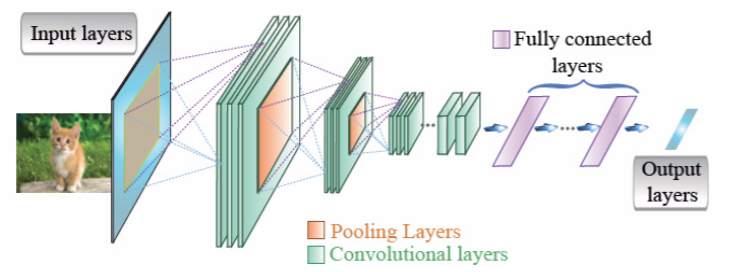
\includegraphics[scale=0.7]{CNN}
\caption{Convolutional Neural Network}
\end{figure}
A convolutional neural network (CNN) consists of three types of layers: \textit{full-connected layers, convolutional layers, and pooling layers}. Fully-connected layers are defined in the same way as a layer in the basic neural network model. Convolutional layers and pooling layers are unique to CNN. A convolution layer in CNN is a composition of two functions: $f^{conv}$ and ${\bm\sigma(x)}$ representing \textit{quasi-convolution} and \textit{activation function} separately. A pooling layer is represented by $f^{pool}$, the \textit{pooling function}. We will provide definitions to these terminologies and function in the following sections.

\section{Basic Tensor Notations}

{\bf Tensor}
\begin{itemize}
\item
Definition of tensor: an multi-dimensional array $\mathcal{F}\in\mathbb{R}^{n_1\times n_2\times\cdots\times n_d}$.
\item
Element-wise representation: 
$$
\mathcal{F}(i_1,...,i_d)\in\mathbb{R}, i_j=0,...,n_j-1, j=1,...,d.
$$
\item
Fiber: mode-1 tensor (vector) obtained by fixing every index but one.
\item
Slice: mode-2 tensor (matrix) obtained by fixing every index but two.
\item
Tensor Norm: 
$$
\|\mathcal{F}\| := \sqrt{\sum_{i_1=1}^{I_1}\cdots\sum_{i_N=1}^{I_N} \mathcal{F}(i_1,...,i_N)^2}
$$
\end{itemize}
\begin{figure}[ht]
\centering
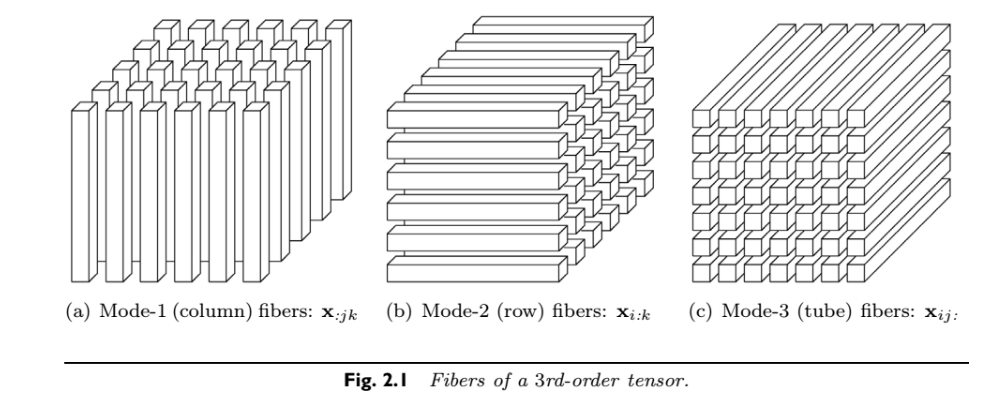
\includegraphics[scale=0.5]{fiber}
\end{figure}
\begin{figure}[ht]
\centering
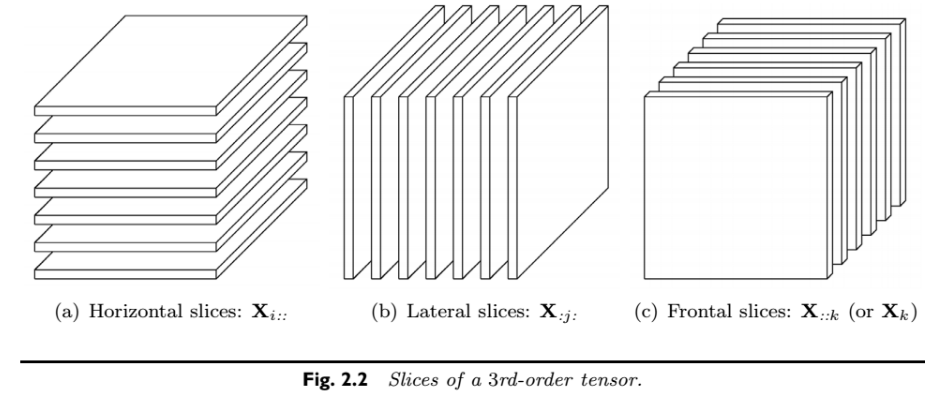
\includegraphics[scale=0.5]{slice}
\end{figure}

{\bf Matricization}.
The mode-$k$ matricization of a tensor $\mathcal{X}\in\mathbb{R}^{n_1\times n_2\times\cdots\times n_d}$ is denoted by $X_{(k)}$ and arranges the mode-$k$ fibers to be the columns of the resulting matrix. Under matricization, the tensor element $\mathcal{X}(i_1,...,i_d)$ is mapped to matrix element $\big(\bm{X_{(k)}}\big)(i_k,j)$, where
\begin{equation}
j = \sum_{1\le s\le d, s\neq k}\big(i_s\prod_{1\le t\le s-1, t\neq k}n_t\big)
\end{equation}
An example is given in Figure \ref{fmat}.
\begin{figure}[H]\label{fmat}
\centering
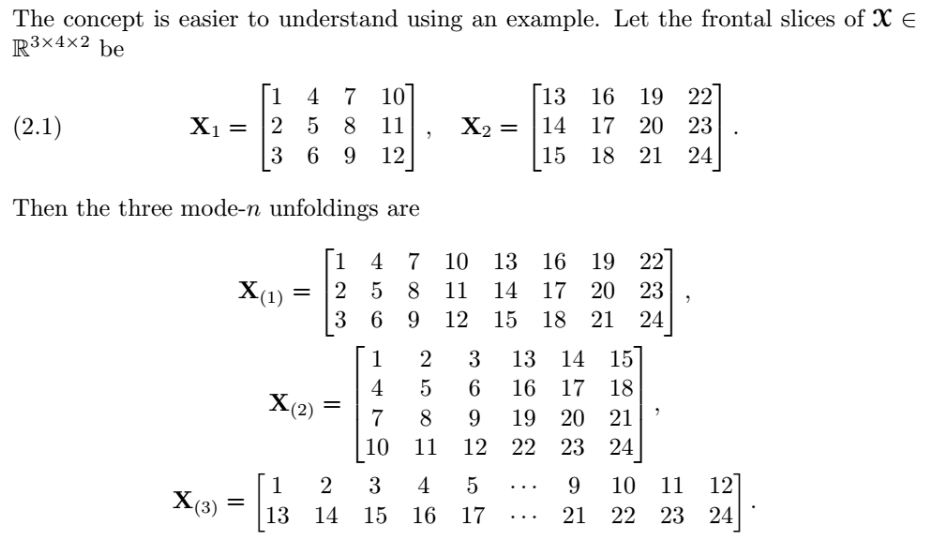
\includegraphics[scale=0.6]{metricization}
\caption{Tensor Matricization}
\end{figure}

%{\bf Tensor-Matrix Multiplication}
Tucker decomposition is best illustrated through \textit{tensor-matrix multiplication}. A product of a tensor $\mathcal{X}$ and a matrix $ M=\big(m_{ij}\big)_{i,j}$ on the $k$-th mode is a tensor defined as:
\begin{equation}
    \big(\mathcal{X}\times_kM\big)[i_1,...,i_n] = 
    \sum_j \mathcal{X}[i_1,...,i_{k-1},j,i_{k+1},...,i_n]m_{ji_k}.
\end{equation}
$M\times_k\mathcal{X}$ can be defined similarly as
\begin{equation}
    \big(M\times_k\mathcal{X}\big)[i_1,...,i_n] = 
    \sum_j m_{i_kj}\mathcal{X}[i_1,...,i_{k-1},j,i_{k+1},...,i_n]m_{i_kj}.
\end{equation}
The following properties are easily provable:
\begin{lemma}
[Tensor-Matrix Multiplication]
\begin{equation}
\aligned
&(\mathcal{X}\times_k M)\times_l N = (\mathcal{X}\times_l N)\times_k M =: \mathcal{X}\times_k M\times_l N\\
&(\mathcal{X}\times_k M)\times_k N = \mathcal{X}\times_k(M\cdot N)
\endaligned
\end{equation}
\end{lemma}

{\bf Tensor Multiplication}.
Given $\mathcal{F}\in\mathbb{R}^{n_1\times\cdots\times n_{d_1}}$, $\mathcal{G}\in\mathbb{R}^{n_1\times\cdots\times n_{d_2}}$, and a mode $k\in\{1,...,\min(d_1,d_2)\}$, the \textit{tensor multiplication on mode $k$} is a tensor such that
\begin{equation}
\aligned
&\big(\mathcal{F}\times_k\mathcal{G}\big)(i_1,...,i_{k-1},i_{k+1},...,i_{d_1},j_1,...,j_{k-1},j_{k+1},...,j_{d_2}) \\
=& \sum_l \mathcal{F}(i_1,...,i_{k-1},l,i_{k+1},...,i_{d_1})\mathcal{G}(j_1,...,j_{k-1},l,j_{k+1},...,j_{d_2}).
\endaligned
\end{equation}
Note that the definition of tensor multiplication can be extended to multiplication on multiple modes.

\section{Quasi-Convolution in CNN}
The mathematical convolution is a operation on two functions ($f$ and $g$); it produces a third function, that is typically viewed as a modified version of one of the original function.

\begin{itemize}
\item
Continuous convolution
$(f*g)(x) := \int_{-\infty}^{\infty}f(t)g(x-t)dt$
\item
Discrete convolution
$(f*g)[n] := \sum_{-\infty}^\infty f[m]g[n-m]$
%\item
%Two-Dimensional convolution
%$(F*G)[i,j] := \sum_{s = -\infty}^\infty\sum_{t = -\infty}^\infty F[s, t]G[i-s, j-t]$
\item 
d-Dimensional convolution
$$(\mathcal{F}\ast \mathcal{G})(i_1, i_2, \cdots ,i_d) = \sum_{j_i, j_2,\cdots,j_d \in \mathbb{Z}} \mathcal{F}(j_1, j_2,\cdots,j_d)\mathcal{G}(i_1 - j_1, i_2 - j_2, \cdots, i_d - j_d)$$
\end{itemize}

\begin{lemma}[Commutativity of Tensors]\label{lconv}
$\mathcal{F}\ast \mathcal{G} = \mathcal{G}\ast \mathcal{F}$.
\end{lemma}

The convolution of two finite-dimensional tensors is defined by extending the sequences to finitely supported functions on the set of integers. In order to understand the computation of a convoltional layer, we need to define a \textit{reversed tensor} and a \textit{quasi-convolution}. A reversed tensor $rev(\mathcal{F})$ of a tensor $\mathcal{X}$ is a tensor with elements in the reversed order, namely
\begin{equation}\label{erevt}
rev(\mathcal{F})(i_1,i_2,...,i_d) := \mathcal{F}(-i_1,-i_2,...,-i_d), i_1,...,i_d\in\mathbb{Z}.
\end{equation}

Moreover, for two tensors $\mathcal{F}\in\mathcal{R}^{n_1\times\cdots\times n_d}$ and $\mathcal{G}\in\mathcal{R}^{m_1\times\cdots\times m_d}$ with $n_1\ge m_1,...,n_d\ge m_d$, we define a \textit{quasi-convolution} $\mathcal{F}\odot\mathcal{G}$ as a truncated convolution of $\mathcal{F}$ and $rev(\mathcal{G})$:
\begin{equation}
\label{eqconv}
\mathcal{F}\odot\mathcal{G} := \big(\mathcal{G}\ast rev(\mathcal{F})\big)(0:(n_1-m_1), 0:(n_2-m_2),...,0:(n_d-m_d))\in\mathbb{R}^{(n_1-m_1+1)\times\cdots\times(n_d-m_d+1)}.
\end{equation}
\begin{lemma}
\label{lqconv}
Let $\mathcal{F}\in\mathcal{R}^{n_1\times\cdots\times n_d}$ and $\mathcal{G}\in\mathcal{R}^{m_1\times\cdots\times m_d}$ with $n_1\ge m_1,...,n_d\ge m_d$. Then their quasi-convoltion $\mathcal{H}:=\mathcal{F}\odot\mathcal{G}$ can be computed as
\begin{equation}
\mathcal{H}(i_1,...,i_d) =
\sum_{0\le j_1\le m_1-1}\cdots\sum_{0\le j_d\le m_d-1}\big(\mathcal{F}(i_1+j_1,...,i_d+j_d)\mathcal{G}(j_1,...,j_d)\big).
\end{equation}
\end{lemma}
In CNN, the input of a convolutional layer is a 3-mode tensor $\mathcal{X}\in\mathbb{R}^{n_1\times n_2\times n_3}$, usually visualized as a collection of $n_3$ matrices of size $n_1\times n_2$. Each such matrix is refered to as an \textit{input channel}. The kernels of a convolutional layer forms a 4-mode tensor $\mathcal{K}\in\mathbb{R}^{d\times d\times n_3\times n_4}$. The function is defined as a quasi-convolution
\begin{equation}
\label{econv}
\aligned
f^{conv}(\mathcal{X}, \mathcal{K}) =& \mathcal{Y}\in\mathbb{R}^{(n_1-d+1)\times (n_2-d+1)\times n_4},\\
\mathcal{Y}(:,:,l) :=& \big(\mathcal{X}\odot\mathcal{K}(:,:,:,l)\big)(:,:,0).
\endaligned
\end{equation}
\begin{lemma}[Express $f^{conv}$ through 2D-convolutions]
Let $\mathcal{X}\in\mathbb{R}^{n_1\times n_2\times n_3}$, $\mathcal{K}\in\mathbb{R}^{d\times d\times n_3\times n_4}$, and $f^{conv}(\mathcal{X}, \mathcal{K}) = \mathcal{Y}\in\mathbb{R}^{(n_1-d+1)\times (n_2-d+1)\times n_4}$. Then
\begin{equation}
\label{e2dconv}
\mathcal{Y}(:,:,l) = \sum_{k=0}^{n_3-1}\big(\mathcal{X}(:,:,k)\odot\mathcal{K}(:,:,k,l)\big).
\end{equation}
A slice $\mathcal{Y}(:,:,l)$ is sometimes called a \textit{feature map}.
\end{lemma}


Two-dimensional quasi-convolution can be visualized as in Figure \ref{fconv}. Here the kernel slides though the entire input matrix.
\begin{figure}[ht]
\label{fconv}
\centering
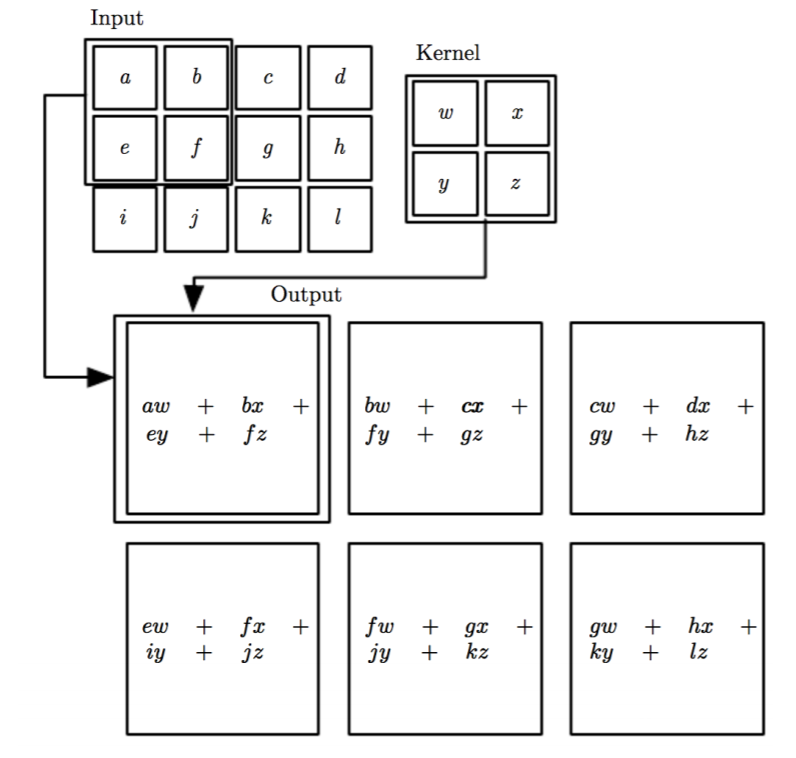
\includegraphics[scale=0.4]{Convolution1}
\caption{Convolution in CNN}
\end{figure}


\section{Convolution via Fast Fourier Transform}

{\bf Discrete Fourier Transform (DFT)}. For a positive integer $n$, the \textit{Fourier transform matrix of degree $n$} is define as the following $n\times n$ matrix
\begin{equation}
\Omega_n:=\big(\omega_n^{-ij}\big)_{i,j}=\frac{1}{\sqrt{n}}\left[
\begin{array}{cccc}
\omega_n^0 & \omega_n^0 & \cdots & \omega_n^0\\
\omega_n^0 & \omega_n^{-1} & \cdots & \omega_n^{-(n-1)}\\
\vdots	& \vdots & & \vdots\\
\omega_n^0 & \omega_n^{-(n-1)} & \cdots & \omega_n^{-(n-1)^2}
\end{array}
\right],
\end{equation}
where $\omega_n = exp(\frac{2\pi i}{n})$. For an $n$-dimensional vector $\bm v = (v_0,...,v_{n-1})$, its \textit{discrete Fourier transform} is defined as 
\begin{equation}
fft(\bm v):=\Omega_n\bm v.
\end{equation}
Similarly, for an $m\times n$ matrix $X$, its \textit{2-dimensional discrete Fourier transform} is defined as
\begin{equation}
2Dfft(X):= \Omega_m X \Omega_n.
\end{equation}
We have the following lemma for the inverse of Fourier transform.
\begin{lemma}
The inverse of 1D DFT is:
\begin{equation}
ifft(\bm v) = \Omega^{-1}\bm v = \Omega^H\bm v.
\end{equation}
The inverse of 2D DFT is:
\begin{equation}
2Difft(X) = \Omega_m^{-1} X \Omega_n^{-1} = \Omega_m^H X \Omega_n^H.\
\end{equation}
Here $X^H$ denotes the hermitian transpose.
\end{lemma}

{\bf DFT and convolution}. Discrete convolution can be achieved by DFT, element-wise multiplication, and inverse DFT.
\begin{lemma}
Let $F, G\in\mathbb{R}^{n_1\times n_2}$, then
\begin{equation}
(F\ast G) = 2Difft(2Dfft(F)\circ 2Dfft(G)).
\end{equation}
Here $\circ$ denotes matrix element-wise multiplication.
\end{lemma}

{\bf Fast Fourier transform (FFT)}.
For $n=2^h$, the matrix-vector multiplication $\Omega_n\bm v$ has complexity $O(n\log n)$ if one applies the following lemma recursively:
\begin{lemma}
Let $h\ge 1$ be an integer, $n=2^h$, $\omega_n=exp(\frac{2\pi i}{n})$, and $D = diag(1, \omega,...,\omega^{2^{h-1}-1})$. Then
\begin{equation}
\Omega_n = \left[
\begin{array}{cc}
I_{n/2} & \\
 & D
\end{array}
\right]\cdot
\left[
\begin{array}{cc}
I_{n/2} & I_{n/2}\\
I_{n/2} & -I_{n/2}
\end{array}
\right]\cdot
\left[
\begin{array}{cc}
\Omega_{n/2} &\\
 & \Omega_{n/2}
\end{array}
\right].
\end{equation}
\end{lemma}
By applying this "divide-and-conquer" method, the complexity of 1D DFT and 2D DFT can be reduced to $O(n\log n)$ and $O(mn\log m\log n)$, respectively. Later in this chapter we will show that FFT can be used to accelerate the training of CNN.

\section{Pooling Layer}

{\bf Pooling layer}. Pooling layer subsamples statistics to obtain summary statistics that are invariant to shifts and distortions in some degree. More precisely we have
\begin{equation}
f^{pool}(\mathcal{X}(:,:,l))(i,j) = f(\mathcal{X}(2i-1:2i,2j-1:2j,l)),
\end{equation} 
where commonly used functions $f$ are
\begin{enumerate}
\item
Mean pooling: $f^{mean}(\mathcal{Z})=\big(\frac{\sum_k z_k}{m}\big)$
\item
Max pooling: $f^{max}(\mathcal{Z})=\big(\max_k\{z_k\}\big)$
\item
$l^p$ pooling: $f^{lp}(\mathcal{Z})=\big(\|(z_1,...,z_m)\|_p\big)$
\end{enumerate}
The partial derivative of the pooling function is usually called the \textit{upsample} function $f^{upsample}$. For example. for the max pooling function, the corresponding upscale function is $\mathbbm{1}_{z = \max_k\{z_k\}}$ (distributing the gradient to the entry with maximum value). 

Figure \ref{ffea} illustrates features extracted the first three convolutional Layers  on a facial recognition task.

\begin{figure}[ht]
\label{ffea}
\centering
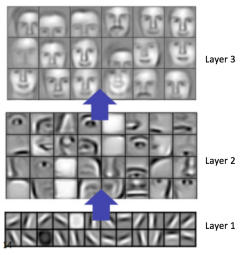
\includegraphics[scale=1]{Features}
\caption{Features}
\end{figure}

\section{Training CNN}
For simplicity, assume that there are no fully-connected layers and there are $D$ convolutional layers and $D$ pooling layers in the CNN model with $f^{conv}$ and $f^{pool}$ defined as in the previous sections. Choose an activation function $\sigma$. Let $S=\{(\mathcal{X}^1, \mathcal{Y}^1),...,(\mathcal{X}^N, \mathcal{Y}^N)\}$ be the training data set. For $(\mathcal{X}, \mathcal{Y})\in S$, the feedforward process $f(\mathcal{X};\mathcal{K}_1,...,\mathcal{K}_D)$ can be described progressively as
\begin{equation}
\aligned
\mathcal{X}_1 =& \mathcal{X}\\
\mathcal{Y}_{i}(\mathcal{X};\mathcal{K}_1,...,\mathcal{K}_i) :=& f^{conv}(\mathcal{X}_i(\mathcal{X};\mathcal{K}_1,...,\mathcal{K}_{i-1}), \mathcal{K}_i)\\
\mathcal{Z}_i(\mathcal{X};\mathcal{K}_1,...,\mathcal{K}_i) :=& \bm\sigma(\mathcal{Y}_{i}(\mathcal{X};\mathcal{K}_1,...,\mathcal{K}_i))\\
\mathcal{X}_{i+1}(\mathcal{X};\mathcal{K}_1,...,\mathcal{K}_i) :=& f^{pool}(\mathcal{Z}_i(\mathcal{X};\mathcal{K}_1,...,\mathcal{K}_i)), i=1,...,D\\
f(\mathcal{X};\mathcal{K}_1,...,\mathcal{K}_D):=&\mathcal{X}_{D+1}(\mathcal{X};\mathcal{K}_1,...,\mathcal{K}_D).
\endaligned
\end{equation}

Then choose a loss function $L(\mathcal{X},\mathcal{Y};\mathcal{K}_1,...,\mathcal{K}_D)$. The goal of training is to minimize the total loss 
\begin{equation}
L_{total}(\mathcal{K}_1,...,\mathcal{K}_D) = \sum_{i=1}^N L(\mathcal{X}^i,\mathcal{Y}^i;\mathcal{K}_1,...,\mathcal{K}_D)
\end{equation}
In order to reduce the number of computations, the \textit{stochastic gradient descent} method samples a subset $S'$ of $S$ (called \textit{mini-batch}) with $|S'|\ll |S|$ and use the following loss function to approximate $L_{total}$:

\begin{equation}
L_{SGD}(\mathcal{K}_1,...,\mathcal{K}_D) = \sum_{(\mathcal{X},\mathcal{Y})\in S'} L(\mathcal{X},\mathcal{Y};\mathcal{K}_1,...,\mathcal{K}_D)
\end{equation}
The gradient of $L_{SGD}$ is the sum of all the corresponding gradients of $L(\mathcal{X},\mathcal{Y})$. 

\begin{figure}[ht]\label{fcnnbp}
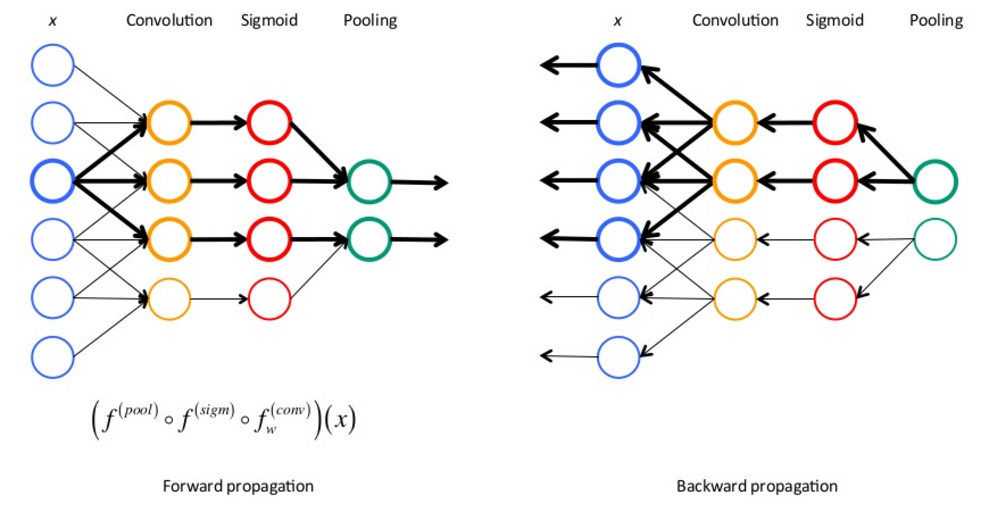
\includegraphics[scale=0.5]{CNNBP}
\caption{Convolutional Layer}
\end{figure}

The backpropagation process can be described as (see Figure \ref{fcnnbp}):
\begin{equation}
\aligned
\delta_{D+1} :=& \frac{\partial L}{\partial \mathcal{X}_{D+1}}\\
\delta_i^{pool} :=&\frac{\partial L}{\partial \mathcal{Z}_i} = \delta_{i+1}\times_{1,2,3}\frac{\partial \mathcal{X}_{i+1}}{\partial \mathcal{Z}_i}=\delta_{i+1}\circ f^{upsample}(\mathcal{X}_{i+1})\\
\delta_i^{sig}:=&\frac{\partial L}{\partial \mathcal{Y}_i} = \delta_i^{pool}\times_{1,2,3}\frac{\partial \mathcal{Z}_i}{\partial \mathcal{Y}_i}=\delta_i^{pool}\circ\bm\sigma'(\mathcal{Y}_i)\\
\delta_i :=&\frac{\partial L}{\partial \mathcal{X}_i}= \delta_i^{sig}\times_{1,2,3}\frac{\partial \mathcal{Y}_i}{\partial \mathcal{X}_i}\\
\delta_i(:,:,l) =& \sum_k \delta_i^{sig}\ast\mathcal{K}_i(:,:,k,l)\\
\frac{\partial L}{\partial\mathcal{K}_i} =& \frac{\partial L}{\partial \mathcal{Y}_i}\times_{1,2,3}\frac{\partial \mathcal{Y}_i}{\partial \mathcal{K}_i}\\
\frac{\partial L}{\partial\mathcal{K}_i}(:,:,k,l) =& \mathcal{X}_i(:,:,k)\odot \delta_i^{sig}(:,:,l)
, i=D,D-1,...,1
\endaligned
\end{equation}

%To backpropagate through one convolutional layer and one pooling layer, one need to compute the derivative of three functions:
%\begin{equation}
%\aligned
%\bm\delta^{conv}_{ikl} =& \frac{\partial L}{\partial x_{ikl}} =
%\sum_{j,k,l}\frac{\partial L}{\partial y_{jkl}}\frac{\partial y_{jkl}}{\partial x_{ikl}} = \sum_{k,l=0}^{r-1}\bm\delta^{sig}_{ikl}\\
%\bm\delta^{sig}_{jkl} =& \frac{\partial L}{\partial y_{jkl}} = \sigma'(y_{jkl})\\
%\bm\delta^{pool}_{jkl} =& \frac{\partial L}{\partial z_{jkl}} = \frac{\partial L}{\partial x^{next}_{jkl}}\frac{\partial x^{next}_{jkl}}{\partial z_{jkl}} = \bm\delta^{next, conv}_{jkl}\\
%\frac{\partial L}{\partial f_{ijkl}} =& \sum_{j,k,l}\frac{\partial L}{\partial y_{jkl}}\frac{\partial y_{jkl}}{\partial f_{ijkl}}=\sum_{s,t=0}^{d-1}\bm\delta^{sig}_{jst}x_{i, s+k, t+l}
%\endaligned
%\end{equation}
Finally, the kernels are updated by the gradient as
\begin{equation}
\mathcal{K}_i \leftarrow \mathcal{K}_i - \eta\frac{\partial L}{\partial\mathcal{K}_i}.
\end{equation}
Note that the complexity of the training process is dominated by the convolution operation in the forward and backward passes.


\section{FFT Based Backpropagation}

Recall that convolution is equivalent to element-wise product in the Fourier form. Typically, this method is used when the size of the convolution kernel is close to that of the input image. Note that a convolution of an image of size $n\times n$ with a kernel of size $d\times d$ using the direct method requires $(n - d + 1)^2d^2$
 operations. The complexity of the FFT-based method requires $(6Cn^2\log n+4n^2)$ operations. Here $C$ represents the constant overhead of FFT. Thus it is not preferable to use FFT for a single convolution in CNN training.
 
However, notice that each channel $\mathcal{X}(:,:,l)$ and each 2D kernel $\mathcal{K}(:,:,k,l)$ appears in $2n$ different convolutions in a forward pass and a backward pass, and one single FFT is sufficient for each matrix. Also notice that from equation (10) only the summation is needed, rather than the convolution results for each summand, suggesting that one can take the sum first and then perform the inverse FFT. Under these two considerations, the total complexity of the training process with FFT is lower than the direct convolution computation.

\begin{figure}[H]
\centering
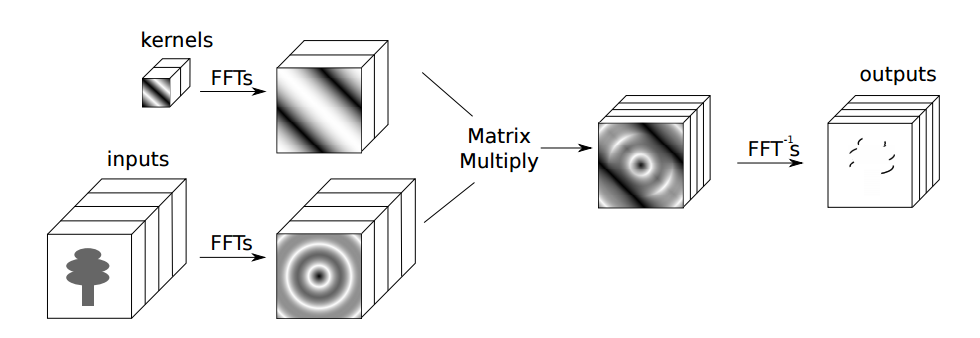
\includegraphics[scale=0.5]{FFTconv}
\caption{Illustration of the FFT based convolution}
\end{figure}

% {\bf Other Implementation Details(future topics)}
% \begin{itemize}
% \item Random sampling
% \item Normalizing the inputs
% \item Choice of activation function
% \item Choosing target values
% \item Initialization
% \item Adaptive learning rates
%\end{itemize}
